\chapter{Topology}

\thispagestyle{standard}
\pagestyle{standard}

The following topology (figure \ref{img:topo}, taken from Moodle instructions) had to be recreated in the lab.

\begin{figure}[H]
	\centering
	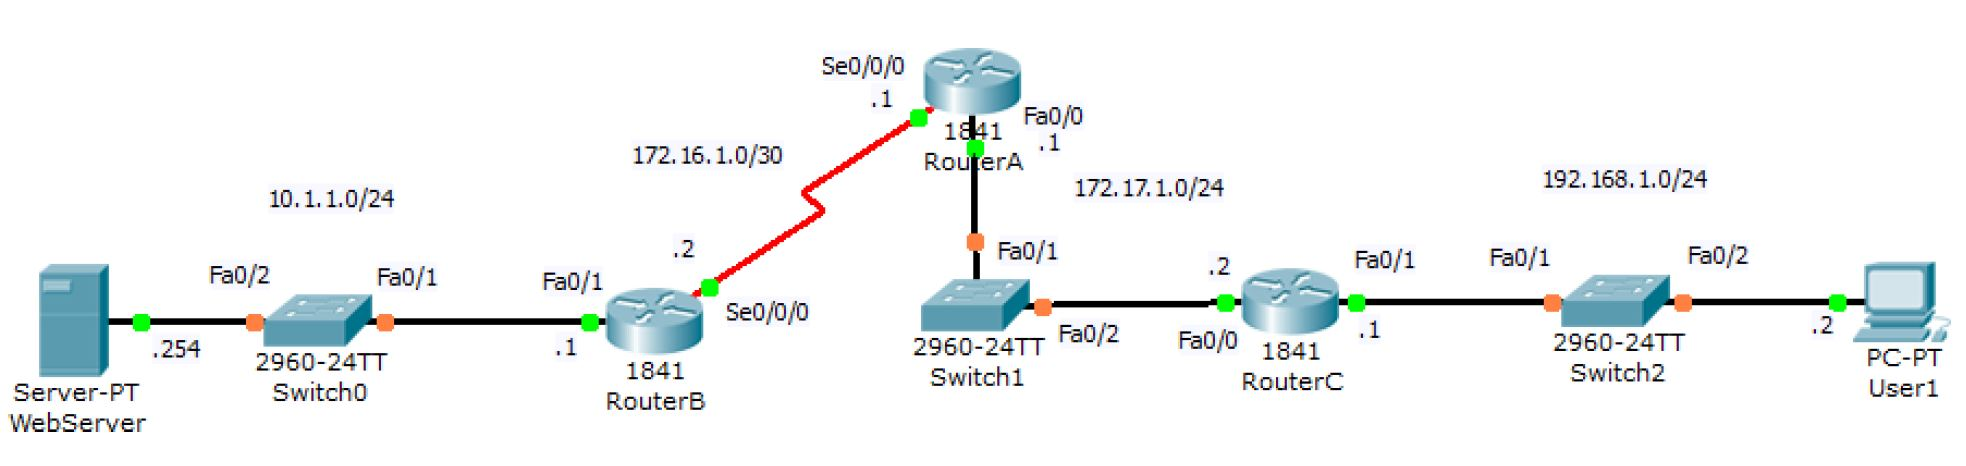
\includegraphics[width=0.9\textwidth]{img/topo.png}
	\caption{Topology (Moodle)}
	\label{img:topo}
\end{figure}

Each device was configured with basic settings like hostname, \ac{MOTD}, a secret enable password, disabled IP domain lookup, synchronous logging on line console 0 and the service password-encryption, which prevents passwords from being displayed in clear-text in the start-up and running configuration. The important part is that the clock-rate for the serial interface has to be configured on the \ac{DCE} device.

\lstset{escapeinside={\%*}{*)},numbers=left}%oder numbers=left
\begin{lstlisting}[caption={Setting the clock-rate on Router A},label={lst:clockrate},language={}]
interface Serial0/0/0
 bandwidth 64
 ip address 172.16.1.1 255.255.255.252
 clock rate 64000
\end{lstlisting}

\ac{OSPF} is a routing protocol for \ac{IP} networks. It uses a \ac{LSR} algorithm and falls into the group of interior routing protocols, operating within a single \ac{AS}.
Concerning the \ac{OSPF} routing, every router assigns its known networks to the \ac{OSPF} routing process with area 0.
\newpage
\lstset{escapeinside={\%*}{*)},numbers=left}%oder numbers=left
\begin{lstlisting}[caption={\ac{OSPF} routing example router A},label={lst:ospf},language={}]
router ospf 1
 area 0 authentication message-digest
 network 172.16.1.0 0.0.0.3 area 0
 network 172.17.1.0 0.0.0.255 area 0
\end{lstlisting}

`nginx' has been set up as a webserver on a Linux-PC. The default `index.html' was adapted to show the message \texttt{"Guter Webserver!"} when accessing the server via a web browser. \\
The IP address has been assigned to `10.1.1.254'.
Ping and webserver access from the User-PC to the server has been successful as shown in (figure \ref{img:GuterWebserverScreenshot}). The firewall on the Windows machines was disabled to prevent accidental ICMP failures.

\begin{figure}[H]
	\centering
	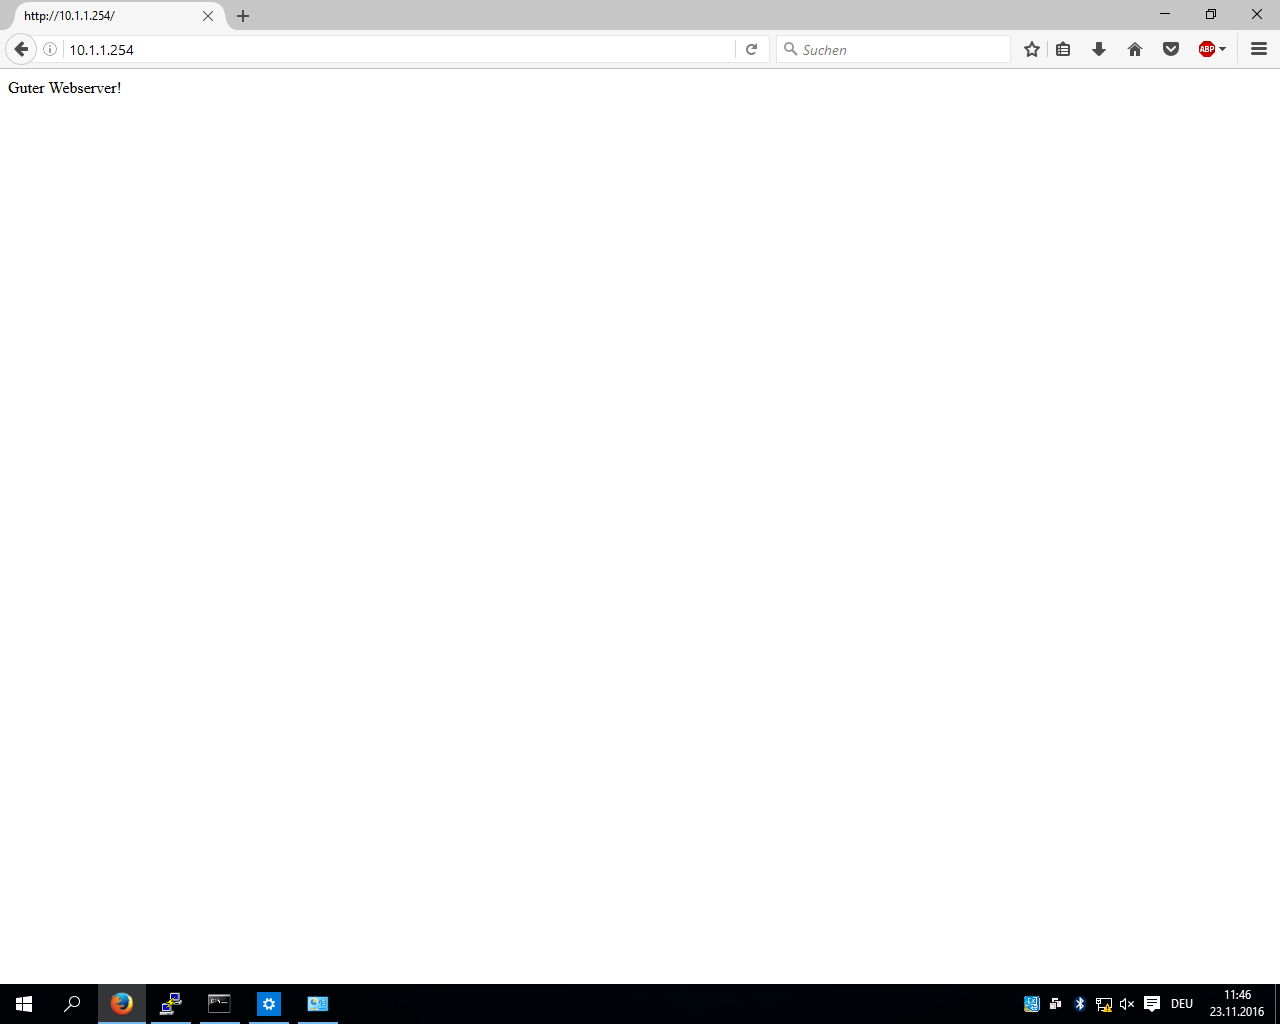
\includegraphics[width=1.0\textwidth]{img/GuterWebserverScreenshot.png}
	\caption{Webserver access}
	\label{img:GuterWebserverScreenshot}
\end{figure}

For this topology the ping command from the user PC to the Linux-PC hosting the webserver took on average of 18ms and had a remaining \ac{TTL} value of 61.
The `tracert' output as shown in (figure \ref{img:TracertGuterWebserver}) from the user PC to the server shows that it takes 4 hops to reach the server.

\begin{figure}[H]
	\centering
	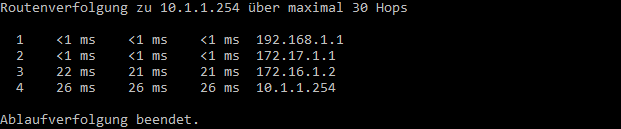
\includegraphics[width=1.0\textwidth]{img/TracertGuterWebserver.png}
	\caption{Tracert from user pc to good webserver}
	\label{img:TracertGuterWebserver}
\end{figure}

\chapter{Router Spoofing}

For the router spoofing attack another router has been added to the network as seen in (figure \ref{img:Router spoofing topology}, taken from Moodle instructions). This router also operates in \ac{OSPF} mode. 

\begin{figure}[H]
	\centering
	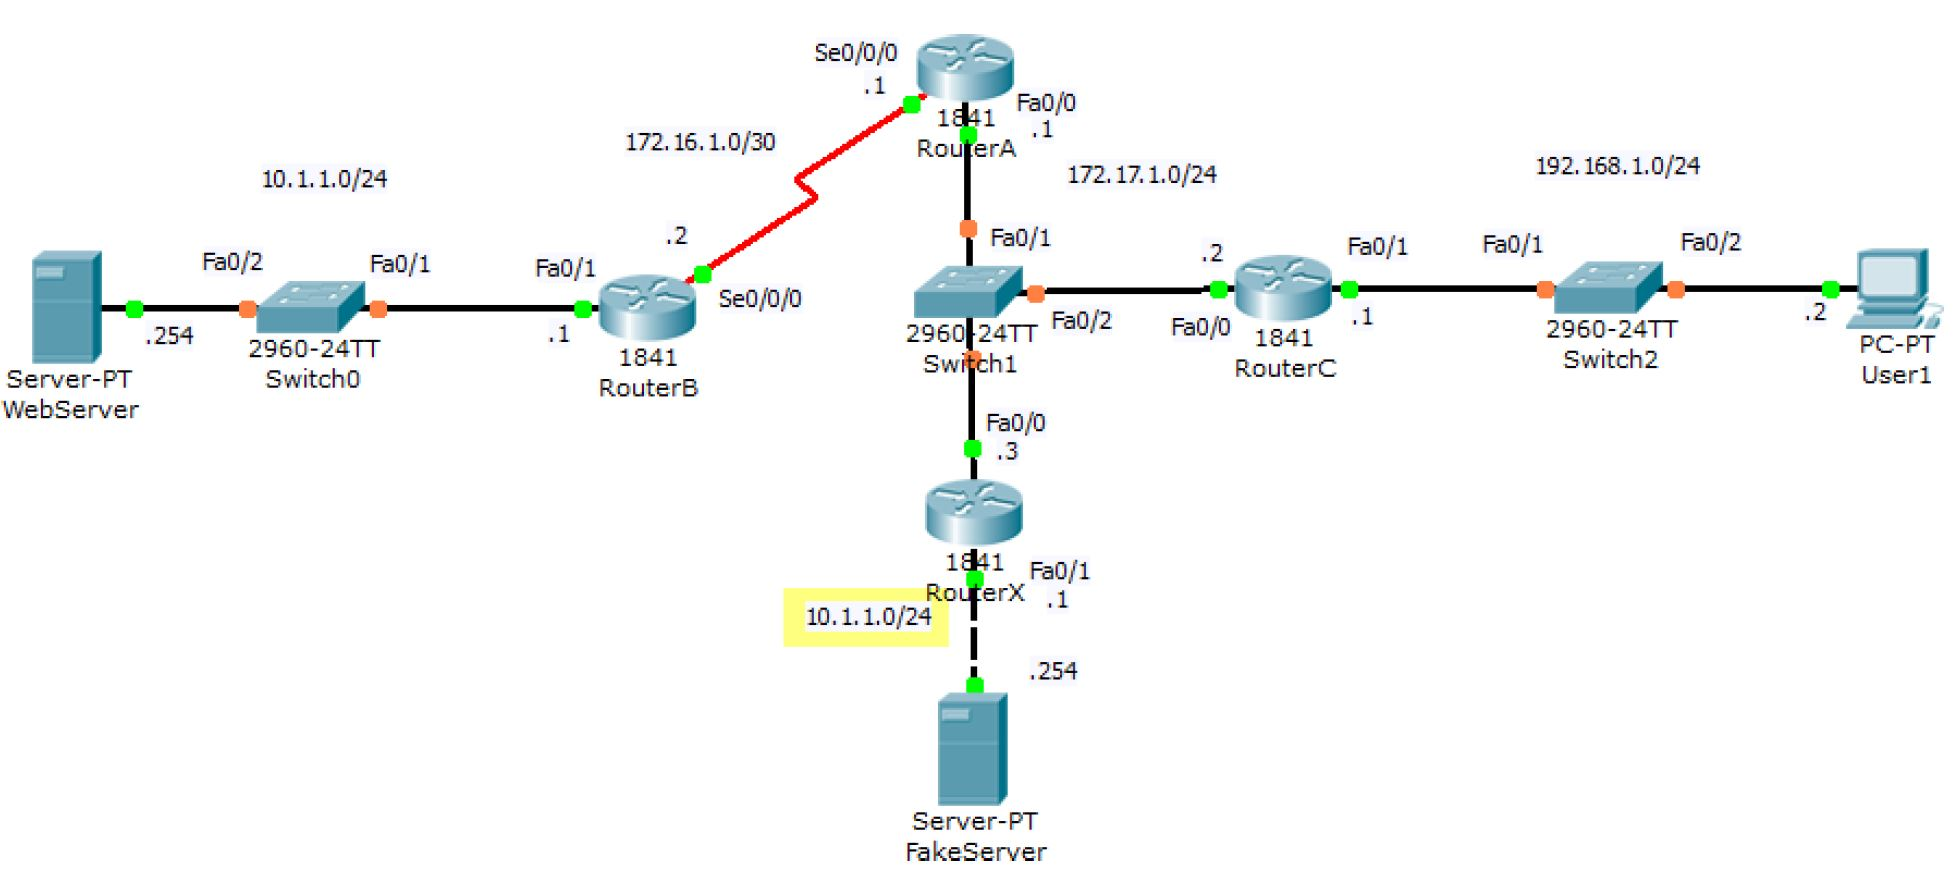
\includegraphics[width=0.9\textwidth]{img/topo_spoofing.png}
	\caption{Router spoofing topology}
	\label{img:Router spoofing topology}
\end{figure}

Router X is now configured to announce the same networks as Router B. The difference between those routers is that Router X is connected via a faster connection (100 Mbps vs. 64 Kbps) then Router B. \\

To also see a difference on the User PC, a second `nginx' was configured on another Linux-PC, this time with \texttt{"Bad Webserver!"} in the `index.html'. 

\lstset{escapeinside={\%*}{*)},numbers=left}%oder numbers=left
\begin{lstlisting}[caption={\ac{OSPF} configuration on router X},label={lst:ospfRouterX},language={}]
router ospf 1
 network 10.1.1.0 0.0.0.255 area 0
 network 172.17.1.0 0.0.0.255 area 0
\end{lstlisting}

\ac{OSPF} detects changes in the topology and computes the shortest-path tree for each route using a method based "Dijkstra's algorithm". The bad Router X propagates that he has a better route to network "10.1.1.0/24". \\
This results in a shorter path from the user pc to the webserver. The user pc doesn't know that this is the bad webserver since \ac{OSPF} only detected a shorter path to the webserver. The router does not know that the two networks, although having the same subnet, are not the same. \\
Therefore, an ICMP Echo request (sent with \texttt{ping}) from the user pc will now be routed to the bad server.
The latency from the user pc to the bad server is now <1ms with a TTL value of 62. Because of the new route the packet isn't sent over the serial link, instead it is being transmitted via the faster Ethernet connection to Router X. The `tracert' output (figure \ref{img:TracertBadWebserver}) shows that the packet only needs 3 hops to its destination and has an average response time of <1ms.

\begin{figure}[H]
	\centering
	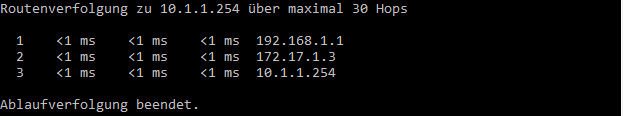
\includegraphics[width=1.0\textwidth]{img/TracertBadWebserver.png}
	\caption{Tracert from user pc to bad webserver}
	\label{img:TracertBadWebserver}
\end{figure}

If the user accesses the webserver again, he will be redirected to the bad webserver, because of the routing table entry in Router C which states that the shortest path to the network "10.1.1.0/24" is reached via Router X.
figure \ref{img:BadWebserverScreenshot} shows the output when accessing the webserver again.

\begin{figure}[H]
	\centering
	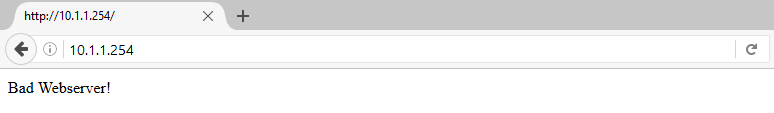
\includegraphics[width=1.0\textwidth]{img/BadWebserverScreenshot.png}
	\caption{Bad webserver access}
	\label{img:BadWebserverScreenshot}
\end{figure}

\chapter{Router Authentication}

In this chapter, router authentication methods are explained. Router authentication for \ac{OSPF} allows to flexibly authenticate \ac{OSPF} neighbours. This enables \ac{OSPF} routing to exchange routing update information in a secure manner.
There are three different types of authentication in OSPF:
\begin{itemize}
\item Null authentication: Also called type 0 -> no authentication information is included in the packet header. This is the default setting.
\item Plain text authentication: type 1 -> use of simple plain-text passwords
\item MD5 authentication: type 2 -> use of MD5 hashed passwords (also not secure anymore!)
\end{itemize}

OSPFv3 is capable of using SHA1 authentication, which is at least better than MD5 authentication.

\section{Plain Text Authentication}

At first, plain text authentication has been configured.
The authentication key is configured for each interface separately by use of the following command:

\texttt{ip ospf authentication-key cisco}

Only interfaces, where the authentication key match, can participate in OSPF advertising.
The following command then enables OSPF authentication for all interfaces inside area 0:

\begin{tabbing}
\texttt{router} \= \texttt{ospf 1} \\
\> \texttt{area 0 authentication}
\end{tabbing}

When the commands above are executed solely on Router A and Router C, all OSPF routes that were advertised from Router B are now lost, because Router B doesn't have the authentication configuration. \\
The main disadvantage of plain text authentication is, that the password can be clearly seen in the packet, as can be seen in figure % \ref{img:}

\pagebreak
\section{MD5 Authentication}

First the MD5 message digest has to be set on the interfaces:
\begin{tabbing}
\texttt{Interf}\= \texttt{ace s0/0/0} \\
\> \texttt{ip ospf message-digest-key 1 md5 cisco}
\end{tabbing}

After that, MD5 authentication can either be enabled on a per interface basis with the following command:
\begin{tabbing}
\texttt{Interf}\= \texttt{ace s0/0/0} \\
\> \texttt{ip ospf authentication message-digest}
\end{tabbing}
   
Or globally for all interfaces belonging to a specific area:
\begin{tabbing}
\texttt{router} \= \texttt{ospf 1} \\
\> \texttt{area 0 authentication message-digest}
\end{tabbing}

\chapter{Sniffing Attack and Clear Text Password Router Authentication}